\section{Experiment} \label{sec:experiment}
We seek to understand the influence of persistent errors on 
FPGA-based neural network acceleration system. Particularly, 
we try to analyze the influence from a system point of view
and figure out the underlying reasons for severe system problems 
such as system stall and dramatic prediction accuracy loss. 

\subsection{Device and Environment}
Xilinx Zynq-7000 SoC ZC706 Evaluation Board will be used in 
the experiments’ hardware implementation. It has 
appropriate hardware resources and is easy to develop and 
use. The hardware design and Bitstream file compilation 
were completed using the upper computer with Intel Core 
i7-6700 processor and 2x8GB DDR4 2400MHz memory. The system 
environment used was Ubuntu 16.04 LTS version, and Xilinx 
Vivado Design Suite and Xilinx Software Development Kits 
version 2017.4.

The hardware resource utilization of the error analysis 
platform implementation on ZC706 is shown in Table \ref{tab:utilization report}.

The four models cover a broad range of applications.
Yolo represent a typical neural network model for object detection \cite{redmon2016yolo9000}, 
Resent is a widely adopted neural network model for classification \cite{He_2016_CVPR}, 
LSTM is the mostly used neural network model for audio classification 
tasks \cite{sak2014long}, and DCGAN stands for a typical neural network model for 
generative tasks \cite{radford2015unsupervised}. 

Despite the widespread adoption of deep learning 
neural network on various applications, it is particularly 
successful in four categories of tasks including object detection, 
object classification, voice recognition and style transfer.
Among a great number of neural network models,
Yolo, Resnet, LSTM and DCGAN are four typical neural networks 
that are comprehensively explored to handle the four computing 
tasks respectively. 

\begin{table}
    \centering
    \caption{Utilization Report of Fault Analysis Platform}
    \label{tab:utilization report}
    \begin{tabular}{cccc}
        \toprule
        Resource & Utilization & Available & Utilization Percentage \\
        \midrule
            LUT & 122618 & 218600 & 56.09\% \\
            LUTRAM & 185 & 70400 & 0.26\% \\
            FF & 84641 & 437200 & 19.36\% \\
            BRAM & 203 & 545 & 37.25\% \\
            DSP & 297 & 900 & 33\% \\
            MMCM & 1 & 8 & 12.5\% \\
        \bottomrule
    \end{tabular}
\vspace{-1em}
\end{table}

\subsection{Overview}
We hope to explore the possible consequences of errors, the 
fault-tolerant ability of different applications and the 
influence of different error locations of accelerators, 
which can provide meaningful references for the subsequent 
network optimization and the fault-tolerant design of 
accelerators.

We conducted five sets of experiments, which explained the 
influence of single error on different networks, the 
difference of fault tolerance ability of different 
applications, the error classification of different 
applications, the influence of different accelerator units 
and whether the input data affected the error representation.


\subsection{Error Consequences and Coverage}
First, we conducted single-bit random error injection 
experiments for different applications, and conducted 
20,000 runs for each application, to analyze the proportion 
of single-bit random error shielded in the system and the 
possible influence of single-bit random error on the 
accelerator system. Figure \ref{fig:lab1-error-rate} shows the 
percentage of application errors caused by a single-bit 
random hardware error. In the experiment, we found that 
more than 90\% of the errors were masked by software or 
hardware. However, while most errors are masked without 
impact to the operation, a single-bit error can lead to 
serious exceptions, including system halt, serious 
deviation in results, and so on. In addition, LSTM network 
has a better fault tolerance performance than other three 
networks, and the proportion of the influence caused by 
single error of the other three networks is about 5~7 times 
that of LSTM. According to our analysis, this is because 
LSTM network is smaller than other networks and uses less 
storage and computing resources.

\begin{figure}
	\center{\includegraphics[width=0.9\linewidth]{lab1-error-rate}}
    \caption{Application error rate caused by single-bit random hardware error}
\label{fig:lab1-error-rate}
\vspace{-0.5em}
\end{figure}


\subsection{Effect of Error Number}
We completed a single run with errors injected number of 
powers of 2, with 20,000 runs for each network. In general, 
the proportion of system halt and result with deviation 
increases with the number of errors, and the accuracy of 
application decreases. Figure \ref{fig:lab2_2} show the proportion of 
system halt and result deviation, and Figure \ref{fig:lab2-network-accuracy} shows the 
accuracy of each network. We found that the influence of 
multiple errors on the accelerator was obvious and far 
beyond our expectation. The Neural Network accelerator is 
still vulnerable to errors. By the time we injected 16 
errors in a single run, the system halt rate was more than 
1\%, means it took more time to restore the system than to 
run it. From the perspective of network accuracy, take YOLO 
system as an example, its mAP decreases by 8.95\% when it 
runs with 16 errors, means the application function of the 
system is also seriously affected.

The result with deviation proportion of different networks 
appears differently with the increase of error number. When 
16 errors are injected, LSTM network still has a small 
result deviation proportion due to its small network 
structure. The proportion of YOLO system is very high, with 
about 70\% of the results showing errors. ResNet is 
relatively low, with only about 35\% result deviation. 
DCGAN network is in between, and about 50\% of the results 
have numerical errors. We believe that the result deviation 
may be related to the structure of the output. The output 
of YOLO system contains more information such as object 
type, location and size of bounding box, etc., and the 
output of ResNet is simple sorting, while the simple output 
is obviously less susceptible to errors.

\begin{figure}
	\center{\includegraphics[width=0.85\linewidth]{lab2-network-accuracy}}
    \caption{Network accuracy versus error number}
\label{fig:lab2-network-accuracy}
\vspace{-0.5em}
\end{figure}

\begin{figure}
    \centering
    \subfigure[System halt]{\includegraphics[width=0.45\linewidth]{lab2-system-halt}}
    \subfigure[Result with deviation]{\includegraphics[width=0.45\linewidth]{lab2-result-with-deviation}}
    \caption{Abnormal situation proportion versus error number}
\label{fig:lab2_2}
\vspace{-0.5em}
\end{figure}


\subsection{Details of Result with Deviation}

\begin{figure*}
    \centering
    \subfigure[YOLO]{\includegraphics[height=0.12\textheight]{lab3-yolo}}
    \subfigure[ResNet]{\includegraphics[height=0.12\textheight]{lab3-resnet}}
    \subfigure[LSTM]{\includegraphics[height=0.12\textheight]{lab3-lstm}}
    \subfigure[DCGAN]{\includegraphics[height=0.12\textheight]{lab3-dcgan}}
\caption{Distribution of result with deviation situations}
\label{fig:lab3}
\vspace{-0.5em}
\end{figure*}

\begin{figure*}
    \centering
    \subfigure[YOLO]{\includegraphics[height=0.10\textheight]{lab4-yolo}}
    \subfigure[ResNet]{\includegraphics[height=0.10\textheight]{lab4-resnet}}
    \subfigure[LSTM]{\includegraphics[height=0.10\textheight]{lab4-lstm}}
    \subfigure[DCGAN]{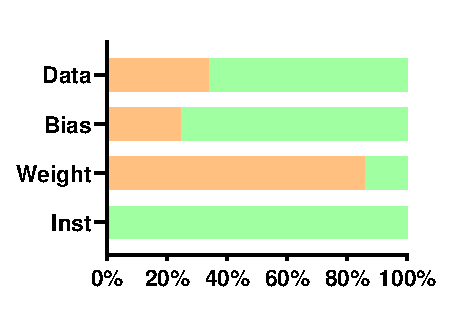
\includegraphics[height=0.10\textheight]{lab4-dcgan}}
    \includegraphics[height=0.10\textheight]{lab4-symbol}
\caption{Proportion of different error location}
\label{fig:lab4}
\vspace{-0.5em}
\end{figure*}

The results with errors are further classified and analyzed. In general, most of the errors are small, with a certain proportion of serious errors and relatively few moderate ones. We believe that most of the errors do not belong to the errors with global influence, but only affect one or several calculations. For example, a single value in the convolution kernel changes. Alternatively, a portion of the error is masked by subsequent calculations such as the max pooling layer. Some errors may have an impact on the control path or the reusable module, resulting in the accumulation of errors throughout the calculation; Or errors that cause serious deviations in the data, such as sign bit upset, can have serious consequences. Figure \ref{fig:lab3} shows the details of result distribution of result with deviation situations.

Specific to each network, about 70\% of the YOLO system's errors belong to the level of bounding box overlap ratio more than 80\%. The total of object type errors and non-overlapping boxes is about 20\%. The remaining 10\% or so is moderate errors. We think this is caused by the implementation of YOLO. YOLO divides the input images into a series of grid cells, and each grid cell is only responsible for one kind of object. Moreover, there is a binary judgment Pr(Object) whether there is a target or not in the confidence degree, which leads to more object type error cases. The bounding boxes that are given after object recognition based on relative wide and high are less sensitive.

More than 70\% of the errors in the ResNet and LSTM classification networks were small impact results of matching four or five items. We think this is because the output is SoftMax layer, which is less affected by the error, and the error is easy to be hidden when sorting, so the result only shows a small alter. However, with the increase of the number of errors, the proportion of serious errors of no matching item in ResNet results increased with the increase of the number of errors and exceeded 10\%. Serious errors cannot be hidden, and the networks fault tolerance for multiple errors is relatively limited.

The result of DCGAN is about 90\% of the results are small deviation level of more than 90\% of SSIM. Only a few of them have a large deviation. Combined with the image, in 90\% of the small deviation results compared with the standard output, basically no difference can be directly seen, and only a few large deviation results have serious distortion of the image. Considering that the output is picture information, these small deviations can be ignored without affecting the visual effect, we believe that DCGAN has relatively strong error tolerance.


\subsection{Effect of Error Location}
In this period, we conducted the experiment results of different error locations. We injected a single-bit random error into a designated location, and conducted multiple experiments to observe the performance of the network. By analyzing the influence of error in different locations on the accelerator, it can provide specific methods for the subsequent fault-tolerant design.

In general, the system is less affected by configuration memory errors, considering that the error injection of configuration memory is global, whose errors may not affect the system. Errors in configuration memory can cause system halt or result with deviation. Errors in BRAMs used for instruction buffer can cause system halt or result with deviation, while BRAMs used in other type buffers can only cause numerical deviations.

We focus on the analysis of the system halt situations caused by error in instruction buffer, which take about 20\% part of the system halt situations. Compared with the instruction before and after upset, the system halts caused by instruction errors includes three situations: instruction type changes, wrong instruction not defined, and the parameter in the operation is abnormal. Different instruction types of the original instruction are considered. Table \ref{tab:instruction change} and Table \ref{tab:original instruction type} shows the detail of instruction error. About 50\% of the system halt situations are caused by the error of DMA instructions. The abnormal access address or boundary violation caused by the abnormal parameters of DMA instruction will lead to the system halt. About 30\% are caused by AGU instruction errors, which result in abnormal in-chip control flow.

\begin{table}
    \centering
    \caption{Instruction change}
    \label{tab:instruction change}
    \begin{tabular}{cc}
        \toprule
            Situation & Percentage \\
        \midrule
            Error instruction undefined & 2.48\% \\
            Instruction type change & 7.45\% \\
            Abnormal parameter & 90.06\% \\
        \bottomrule
    \end{tabular}
\vspace{-1em}
\end{table}

\begin{table}
    \centering
    \caption{Original instruction type}
    \label{tab:original instruction type}
    \begin{tabular}{cc}
        \toprule
            type & Percentage \\
        \midrule
            DMA & 55.90\% \\
            AGU & 32.92\% \\
            others & 11.18\% \\
        \bottomrule
    \end{tabular}
\vspace{-1em}
\end{table}


The proportions of errors in instruction buffer led to system halt in ResNet, YOLO and LSTM, reached 1.15\%, 2.55\% and 4.25\% respectively, seriously affecting the proper application of the system. For result with deviation case, in the experiment of YOLO, about half of the result deviation situations caused by instruction buffer errors were serious object type errors. In the experiment of ResNet, a large number of mismatches were also caused. DCGAN network is limited by instruction errors, because the instruction sequence length of this network is very short, only 2\% of the instruction buffer is used, while the instruction sequence of other networks uses instruction buffer of 50\%\~{}80\%. Combined with the result with deviation and system halt case, we propose that instruction buffer needs to be strengthened in the fault-tolerant design.


Errors in the buffers used in data-flow, such as weights, data, and bias buffer, do not cause system halt, only may cause result deviations. In general, data and weights are more sensitive than bias. Taking YOLO system as an example, the proportion of result deviation caused by single error in weight, data and bias buffer is 48.75\%, 56.95\% and 6.35\% respectively. Horizontal comparison shows that each network has different sensitivity to different buffer errors, as shown in figure {}.


\subsection{Input-Related Error}
In the above experiments, we used different input data for 
experiments, and we verified the relationship between 
errors and input data in this set of experiments. We test 
different input data using the same error. Whether a 
hardware error causes an application error exists in two 
ways, depending on the input data or not. Errors unrelated 
to input data, fixed to cause system halt or result 
deviation, or be masked, that is, different input data will 
not influence the classification of the result. The other 
part of the errors is input data related, which can be 
shown as replacing different input data, result match 
situation and result with deviation situation both appear. 
In other words, different input data has different 
sensitivity to an input-related error. We believe that this 
is caused by structures which error affected. 
Input-unrelated errors may affect the control-flow of the 
system, the bus, etc. These structures are used in every 
operation, and the errors will not be masked by subsequent 
calculations. Input-related errors may affect the relevant 
data in the data-flow, and some errors may be masked in 
the subsequent calculation. Due to the large number of 
experiments, we only observed this phenomenon without 
further study on its proportion and distribution.


